\documentclass[12pt,twoside]{book}
\usepackage{../../thesis}
\usepackage{xfrac}
\graphicspath{ {../../images/} }
\usetikzlibrary{calc}
\tikzset{
    right angle quadrant/.code={
        \pgfmathsetmacro\quadranta{{1,1,-1,-1}[#1-1]}     % Arrays for selecting quadrant
        \pgfmathsetmacro\quadrantb{{1,-1,-1,1}[#1-1]}},
    right angle quadrant=1, % Make sure it is set, even if not called explicitly
    right angle length/.code={\def\rightanglelength{#1}},   % Length of symbol
    right angle length=4pt, % Make sure it is set...
    right angle symbol/.style n args={3}{
        insert path={
            let \p0 = ($(#1)!(#3)!(#2)$) in     % Intersection
                let \p1 = ($(\p0)!\quadranta*\rightanglelength!(#3)$), % Point on base line
                \p2 = ($(\p0)!\quadrantb*\rightanglelength!(#2)$) in % Point on perpendicular line
                let \p3 = ($(\p1)+(\p2)-(\p0)$) in  % Corner point of symbol
            (\p1) -- (\p3) -- (\p2)
        }
    }
}

\makeindex
\begin{document}
\chapter{Outer Billiard}
In this chapter, we illustrate an example of chaotic map, \textit{outer billiards}.
The dynamical system is a one-parameter map on $\R^2$, and for two special cases, we prove that the map is not chaotic in any sense.
For the other vast majority of cases, however, the map seems to be chaotic in some sense.
We present the results from numerical simulations.

\section{The Billiard Map and Kite}
An \textit{outer billiard} is a dynamical system with a simple geometrical interpretation.
An outer billard is a dynamical system $(X, B_S)$, where $X$ is a set of points in $\R^2$, and $B_S$ is a \textit{billiard map} determined by a \textit{shape} $S$.
Unlike the billiards game that we are familiar with, the points (or balls) move around outside the shape (or table).
For any given point $p$, if the point is inside or on $S$, then $B_S$ maps $p$ to itself.
If $p$ is outside the kite, on the other hand, $B_S$ maps $p$ to $q$, where $q$ is a point such that $\overline{pq}$, the line segment between $p$ and $q$, is tangent to $S$, and $\overline{pq}$ intersects $S$ at the midpoint of $\overline{pq}$ (Figure~\ref{fig:billiards}).
\begin{figure}[ht]
  \centering
  \begin{tikzpicture}[scale=3,cap=round]
  % Local definitions
  %\def\costhirty{0.9660256}

  % Colors
    \colorlet{anglecolor}{green!20!black}

  % Styles
    \tikzstyle{axes}=[]

  % The graphic
  %grid
  %\draw[style=help lines,step=0.5cm] (-1.4,-1.4) grid (1.4,1.4);

    \draw (0,0) circle (1cm) coordinate (o);
    \draw [fill=red] (1.333,2) circle [radius=0.05] coordinate (p);
    \draw [fill=green] (-2.385,-0.2988) circle [radius=0.05] coordinate (q);
    \draw [fill] (-0.5258, 0.8506) circle [radius=0.01] coordinate (t);

    \begin{scope}[style=axes]
      \draw[->] (-2,0) -- (2,0) node[right] {$x$};
      \draw[->] (0,-1.5) -- (0,1.5) node[above] {$y$};

      \foreach \x/\xtext in {1}
      \draw[xshift=\x cm] (0pt,1pt) -- (0pt,-1pt) node[below,fill=white]
      {$\xtext$};

      \foreach \y/\ytext in {-1}
      \draw[yshift=\y cm] (1pt,0pt) -- (-1pt,0pt) node[left,fill=white]
      {$\ytext$};
    \end{scope}

    \draw[draw=anglecolor] (0.2,0.3) arc (56.31:121.73:0.36cm);
    \draw (80:5mm) node[anglecolor] {$\phi$};
%  \draw[draw=anglecolor] (121.73:0.20cm) arc (121.73:187.15:0.20cm);
%  \draw (160:3.5mm) node[anglecolor] {$\phi$};

    \draw[] (-2.385,-0.2988) --
    node {} (intersection of 0,0--2,3 and 1,2--2,2);

    \draw (0,0) -- (p);
    \draw (0,0) -- (q);
    \draw (0,0) -- (t);
    \draw [right angle symbol={p}{t}{o}];
  \end{tikzpicture}
  \caption{
    An example of an billiard on a unit circle.
    The red ball in the first quadrant gets mapped to the other (green) ball.
  }
  \label{fig:billiards}
\end{figure}

There are necessarily two tangent lines: ones that go around the shape in the counter-clockwise and clockwise directions.
We choose the counter-clockwise one to define the billiard map.

This dynamical system was popularized by Jürgen Moser as a toy model of celestial mechanics~\citep{moser,moserbook}.
We can interpret the shape as the Sun, and the points as planets orbiting the Sun.
The Moser-Neumann question asks if there is an outer billiard system that has a point whose orbit is unbounded.
In an analogy to the Solar system, an unbounded orbit correspond to a planet escaping the system.
\citet{moser} says that the Moser-Neumann question is
``a very simple geometrical problem that actually contains some of the difficulties of the $n$ body problem and may serve as a crude model for planetary motion.''
Regardless of the legitimacy of his claim, the Moser-Neumann question is an interesting mathematical problem with an intriguing geometrical nature (See Figure).
%a tried and true technique of mathematics to extract the essential properties of a problem and to idealize it
\citet{moserbook} showed that an outer billiard on $S$ (the shape) does not have an unbounded orbit provided that $S$ is at least $C^6$ smooth and has positive curvature. 
\citet{schwartz} studies outer billiards when the shape is a Penrose kite, and shows that outer billiards for particular Penrose kites have unbounded orbits.
Other known results are listed in \citet[p. 2]{schwartz}.

In this chapter, we study a family of one-parameter shapes, which we will refer to as \textit{kites}.
\footnote{This family of shapes was suggested by Ray Mayer. Reed College, Portland, OR !ask for permission}
The kites that we study have, unlike the Penrose kites that Schwartz studies, curved edges.
We only consider kites with symmetries of a square.
\begin{definition}
  (Kite $S_d$)
  Let $S_d$ be a shape with one parameter $d$ constructed as follows.
  Let $C_1$ be an arc for $\theta \in (\pi/4, 3\pi/4)$ of a circle of radius $1+d$ centered at $(0,-d)$.
  Rotate $C_1$ by $\pi/4$ around the origin to obtain $C_2$.
  Similarly obtain $C_3$ and $C_4$ by rotations by $\pi/4$.
  Then, let $S_d = C_1 \cup C_2 \cup C_3 \cup C_4$ (See Figure~\ref{fig:kiteeg}).

  We already defined $B_{S_d}$ for any convex shape at the beginning of this chapter, but let us re-iterate the description here.
  We define $B_{S_d}$, the corresponding billiard map, as follows.
  For any given point $p$, if the point is inside or on $S_d$, then $B_{S_d}$ maps $p$ to itself.
  If $p$ is outside the kite, then $B_{S_d}$ maps $p$ to $q$, where $q$ is a point such that $\overline{pq}$, the line segment between $p$ and $q$, is tangent to $S_d$, and $\overline{pq}$ intersects $S_d$ at the midpoint of $\overline{pq}$ (Figure~\ref{fig:kite-regions}).
  We refer to $S_d$ as a \textit{kite}.

\end{definition}
\begin{figure}[ht]
  \begin{center}
    \includegraphics[width=0.8\textwidth]{kite_d10}
    \caption{An example of a kite. The kite shown here is $S_d$ for $d = 1.0$.}
    \label{fig:kiteeg}
  \end{center}
\end{figure}
\begin{figure}[ht]
  \begin{center}
    \includegraphics[width=0.8\textwidth]{kite_w_regions}
    \caption{The kite for $d = 1.0$ with tangent lines at the four points on the kite where the shape is not smooth.}
    \label{fig:kite-regions}
  \end{center}
\end{figure}

\section{Special Case (1): $d = 0$}
\begin{figure}[ht]
  \begin{center}
    \includegraphics[width=0.8\textwidth]{kite_d0}
    \caption{$d = 0$. The kite is a unit circle.}
    \label{fig:kite-circle}
  \end{center}
\end{figure}
%%%
When $d = 0$, the kite is a unit circle (Figure~\ref{fig:kite-circle}).
We only consider the dynamics of the points that are outside the kite, since the mapping of points in or on the kite is defined to be the identity map.
Consider a point $p = (r, \theta)$ with $r > 1$.
We show that $r$ determines the dynamics of the point.
The billiard map for $p$ is a rotation by $2\phi$, where $\phi = \arccos(1/r)$.
(Note that, for each $R \in \R$, the circle $\setst{(r,\theta)}{r = R}$ is an invariant set of the billiard map.)
If there exist $n, k \in \N^+$ such that $n(2\phi) = 2k\pi$, then $p$ is a $n$-periodic point, since 
\begin{equation*}
  \itr{B_S}{n} = (r, \theta + 2k\pi) = (r, \theta).
\end{equation*}
We can ensure that the period of $p$ is not less than $n$ by choosing an appropriate pair $n,k$.
Noting that $\phi = \frac{k}{n}\pi$, and $\phi$ must satisfy $0 < \phi < 1/2$, we obtain the following proposition.
\begin{proposition}
  Let $p \in \R^2$ be a point whose polar coordinates is $(r,\theta)$, and define $\phi \ceq \arccos(1/r)$.
  Suppose $\phi = \alpha\pi$ for $0 < \alpha < 1/2$.
  If $\alpha$ is rational, then $p$ is a periodic point.
  Otherwise, $p$ is aperiodic.
\end{proposition}
%%%
We have found that $r$ determines $2\phi$, the angle of rotation.
Next, we want to find values of $r$ for which the corresponding points are periodic.
We have
\begin{equation*}
  \phi = \alpha\pi = \arccos(\frac{1}{r}) 
  \LRar \cos(\alpha\pi) = \frac{1}{r}
  \LRar r = \frac{1}{\cos(\alpha\pi)}.
\end{equation*}
So consider the set
\begin{equation*}
  A = \setst{\frac{1}{\cos(\alpha\pi)}}{0 < \alpha < \frac{1}{2}}.
\end{equation*}
It is easy to see that
\begin{equation*}
  A = \setst{r}{r > 1, r \in \R}.
\end{equation*}
Also consider the set of $r$ for which the corresponding points are periodic
\begin{equation*}
  Q = \setst{\frac{1}{\cos(\alpha\pi)}}{0 < \alpha < \frac{1}{2}, \alpha \in \Q}.
\end{equation*}
We show that the periodic points are dense in the whole space.
\begin{proposition}
  $Q$ is dense in $A$.
  \begin{proof}
  The set of rational numbers in $(0,1/2)$ is dense in $(0,1/2)$.
  Note that the mapping
    \begin{align*}
      f: (0,\frac{1}{2}) &\to (1, \infty)  \\
      \alpha &\mapsto \frac{1}{\cos(\alpha\pi)}
    \end{align*}
  is continuous and surjective.
  It follows that $Q$ is dense in $A$.
  \end{proof}
\end{proposition}
Therefore, periodic points are dense in the space, and, by the same argument, aperiodic points are also dense.
Finally, let us consider the chaoticity of the dynamical system using Devaney's definition.
Once we fix a radius $R$, the circle of radius $R$ centered at the origin is a closed, invariant set of the mapping.
Since $B_{S_0}$ is simply a rotation by a fixed angle for each point in the circle, the mapping is not sensitive to initial conditions.
If the $R$ that we picked happen to satisfy $1/R = \cos(\alpha\pi)$ for some rational $\alpha$, then $B_{S_0}$ is not topologically transitive.
Otherwise, every point on the circle is aperiodic, so the mapping is topologically transitive.
Note that, if we consider two points with slightly different radii, say $p = (r, \theta)$ and $q = (r + \delta, \theta)$, the two points will be separated by some $\epsilon > 0$.
Thus, if we consider the dynamics of an annular region, the dynamical system has a sensitive dependence on initial conditions.
However, it is not chaotic, since a point never leaves the circle it was originally on, so that the map is not topologically transitive.
Hence, the system is not chaotic in Devaney's sense.

\section{Special Case (2): $d \to \infty$}
\begin{figure}[ht]
  \begin{center}
    \includegraphics[width=0.8\textwidth]{kite_d100}
    \caption{$d = 100$. When $d$ is large, the kite is approximately a square.}
    \label{fig:kite-square}
  \end{center}
\end{figure}
%%%
As $d \to \infty$, the kite approaches a square (Figure~\ref{fig:kite-square}).
In this case, a tangent line from a circle to the kite goes through one of the four corners of the square.
We disregard points in the set 
\begin{equation*}
  G \ceq \setst{(x,y)}{x = n \mbox{ or } y = n \mbox{ for some } n \in \N}
\end{equation*}
because the billiard map is not well-defined.
Similarly, we ignore points on the grid, i.e. points of the form $(n,y)$ or $(x,n)$ for some $n \in \N$ and $x,y \in \R$, because each of these points is eventually mapped to a point in $G$.
(However, we could set an arbitrary rule for where points in $G$ are mapped to.
For example, for $p \in G$, we could choose the closest of the four corners of the square to be the midpoint of $p$ and its destination.)
It is easier to understand the structure of the dynamical system if we group together points into squares labeled as in Figure~\ref{fig:grid} and study the dynamics of squares, instead of considering individual points.
\begin{equation*}
  S_n \ceq \setst{\mbox{square with label } (a,b)}{\abs{a} + \abs{b} = n}.
\end{equation*}
Sets in $S_1$, for instance, have the following dynamics:
\begin{equation*}
  (0,1) \mapsto (-1,0) \mapsto (0,-1) \mapsto (1,0) \mapsto (0,1).
\end{equation*}
Thus, each square in $S_1$ is a 4-periodic set when considering the dynamics of sets.
It is easy to verify that each point in $A \in S_1$ is also $4$-periodic.
We can generalize this observation to $S_n$ for any $n$: each square in $S_n$ is a $4n$-periodic set.
Furthermore, each point in $A \in S_n$ is a $4n$-periodic point.
We leave the proof to the reader.

\begin{figure}[ht]
  \centering
  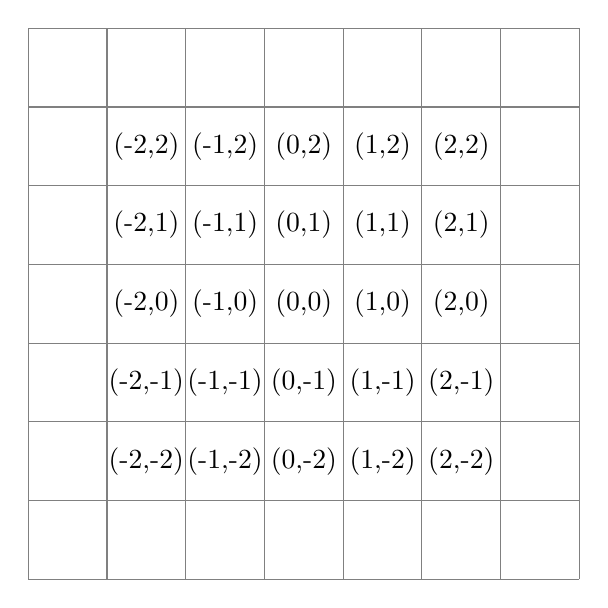
\begin{tikzpicture}
    \draw[step=1.0cm,color=gray] (-4,-4) grid (3,3);
    \node at (-0.5,-0.5) {(0,0)};
    \node at (+0.5,-0.5) {(1,0)};
    \node at (-1.5,-0.5) {(-1,0)};
    \node at (-0.5,+0.5) {(0,1)};
    \node at (-0.5,-1.5) {(0,-1)};
    \node at (+1.5,-0.5) {(2,0)};
    \node at (-2.5,-0.5) {(-2,0)};
    \node at (-0.5,+1.5) {(0,2)};
    \node at (-0.5,-2.5) {(0,-2)};
    \node at (+0.5,+0.5) {(1,1)};
    \node at (-1.5,+0.5) {(-1,1)};
    \node at (+0.5,-1.5) {(1,-1)};
    \node at (-1.5,-1.5) {(-1,-1)};
    \node at (+1.5,+1.5) {(2,2)};
    \node at (-2.5,+1.5) {(-2,2)};
    \node at (+1.5,-2.5) {(2,-2)};
    \node at (-2.5,-2.5) {(-2,-2)};
    \node at (+0.5,+1.5) {(1,2)};
    \node at (-1.5,+1.5) {(-1,2)};
    \node at (+0.5,-2.5) {(1,-2)};
    \node at (-1.5,-2.5) {(-1,-2)};
    \node at (+1.5,+0.5) {(2,1)};
    \node at (-2.5,+0.5) {(-2,1)};
    \node at (+1.5,-1.5) {(2,-1)};
    \node at (-2.5,-1.5) {(-2,-1)};
  \end{tikzpicture}

  \caption{Our naming scheme of grids.}
  \label{fig:grid}

\end{figure}
%%%

\section{Other Cases: $d \neq 0$, $d < \infty$}
So far, we studied the dynamics of the outer billiard system for two particular parameters, which turned out to be fairly simple.
For general cases, however, the dyanamics is considerably more complicated.
We show several results of numerical simulations, and make conjectures about the properties of the system.
However, we have no proof so far for any of the claims that we will make.

The orbits of any points in a bounded set seem to be bounded.
There are periodic points of all periods.
Periodic points of the same periods are clustered together (similar to $d \to \infty$ case).

\begin{figure}[ht]
  \begin{center}
    $
    \begin{array}{l}
      \includegraphics[width=0.45\textwidth]{strip2-3_setup}
    \end{array}
    $\scalebox{2.0}{$\Rar$}$
    \begin{array}{l}
      \includegraphics[width=0.4\textwidth]{strip2-3}
    \end{array}
    $
    \caption{
      The transformation of an annular region between two circles of radius 2 and 3.
      $d = ?$.
      !! Redo the picture on the left in R.
    }
    \label{fig:disk2-3}
  \end{center}
\end{figure}

\begin{figure}[ht]
  \begin{center}
    \includegraphics[width=0.45\textwidth]{strip3-4}
    \includegraphics[width=0.45\textwidth]{strip6-7}
    \caption{Left: transformation of an annular region between two circles of radii 3 and 4.
      Right: between radii 6 and 7.
      $d = ?$.
    }
    \label{fig:disk3-4-6-7}
  \end{center}
\end{figure}

\begin{figure}[ht]
  \begin{center}
    \includegraphics[width=0.6\textwidth]{disk10}
    \caption{Left: transformation of an annular region between two circles of radii 1 and 10.
      Since the billiard map is the identity map for points inside the kite, we can regard this as a transformation of a disk of radius 10.
      $d = ?$.
    }
    \label{fig:disk10}
  \end{center}
\end{figure}

When a point is aperiodic, it seems to be sensitive to initial conditions
Figure~\ref{fig:sensitivity1} shows the evolution of distances between two nearby points.
Initially, the distance between the two points is essentially zero, and the two points remain close to each other in the beginning.
After around 500 iterations, however, the distance between the two starts growing.
The growth ends when the distance is around 9, which seems to be the upper bound.
Then, the two points begin to come close to each other again.
The two points keep distance from each other between 1500-3500 iterations, but starting around 3500th iteration, the distance between the two oscillates between the upper bound and some small value less than 1.
These two points seem to satisfy the criteria of Li-Yorke pair.
Also, there seem to be uncountably many such points (Figure~\ref{fig:strip3-4}).
If these claims turn out to be true, then the system is chaotic in the sense of Li-Yorke.

\begin{figure}[ht]
  \begin{center}
    \includegraphics[width=0.8\textwidth]{billiard_sensitivity_pi-div-10}
    \caption{The evolution of distance between $p = (2, \pi/10)$ and the other point $q$, which is initially close to $p$.
      $q$ was obtained by rotating $p$ by $\epsilon$ radian, where $\epsilon$ is the smallest double available in the precision of the machine.
      The $x$-axis is the number of iterations, and the $y$-axis is the distance between $p$ and $q$.
    }
    \label{fig:sensitivity1}
  \end{center}
\end{figure}

In the cluster of periodic points, the distance between two nearby points shows almost no growth.
\begin{figure}[ht]
  \begin{center}
    \includegraphics[width=0.8\textwidth]{sensitivity_test_slow_growth_45deg}
    \caption{The evolution of distance between $p = (2, \pi/4)$ and the other point $q$, which is initially close to $p$.
      $q$ was obtained by rotating $p$ by $\epsilon$ radian, where $\epsilon$ is the smallest double available in the precision of the machine.
      The $x$-axis is the number of iterations, and the $y$-axis is the distance between $p$ and $q$.
      Even after $5.0 \times 10^6$ iterations, the distance between the two points is on the order of $10^{-1}$.
    }
    \label{fig:sensitivity2}
  \end{center}
\end{figure}

\bibliographystyle{../../bibliography/pjgsm}
\bibliography{../../bibliography/thesis}

\printindex
\end{document}


